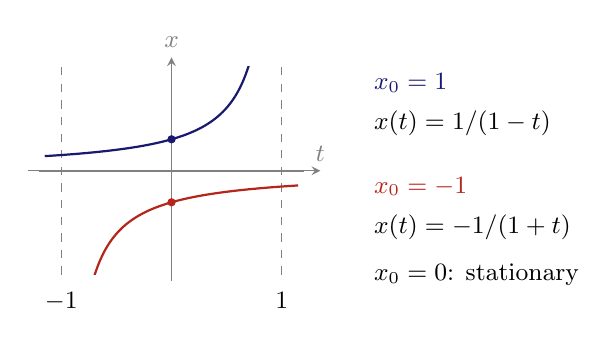
\begin{tikzpicture}[x=1.4cm,y=.4cm,font=\small,>=stealth]
\draw[gray,->] (-1.3,0)--(1.35,0) node[above] {$t$};
\draw[gray,->] (0,-3.5)--(0,3.6) node[above] {$x$};
\draw[gray,dashed] (-1,-3.3)--(-1,3.3);
\draw[gray,dashed] (1,-3.3)--(1,3.3);
\node[below] at (-1,-3.55) {$-1$};
\node[below] at (1,-3.55) {$1$};
\begin{scope}
\clip (-1.2,-3.3) rectangle (1.2,3.3);
\draw[MidnightBlue,thick,domain=-1.15:.96,samples=90] plot (\x,{1/(1-\x)});
\draw[BrickRed,thick,domain=-.96:1.15,samples=90] plot (\x,{-1/(1+\x)});
\draw[gray,thick] (-1.2,0)--(1.2,0);
\end{scope}
\fill[MidnightBlue] (0,1) circle (1.5pt);
\fill[BrickRed] (0,-1) circle (1.5pt);
\node[MidnightBlue,anchor=west] at (1.75,2.8) {$x_0=1$};
\node[anchor=west] at (1.75,1.5) {$x(t)=1/(1-t)$};
\node[BrickRed,anchor=west] at (1.75,-.5) {$x_0=-1$};
\node[anchor=west] at (1.75,-1.8) {$x(t)=-1/(1+t)$};
\node[anchor=west] at (1.75,-3.3) {$x_0=0$: stationary};
\end{tikzpicture}
